\PassOptionsToPackage{numbers,sort&compress}{natbib}
\documentclass{article}

\usepackage[final]{neurips_2025}

\makeatletter
\renewcommand{\@notice}{}
\makeatother

\usepackage[utf8]{inputenc}
\usepackage[T1]{fontenc}
\usepackage{babel}

% \addto\captionsspanish{%
%   \renewcommand{\tablename}{Tabla}%
%   \renewcommand{\figurename}{Figura}%
% }

\usepackage{microtype}
\usepackage{amsmath,amssymb,amsfonts,bm}
\usepackage{booktabs}
\usepackage{multirow}
\usepackage{array}
\usepackage{graphicx}
\usepackage{subcaption}
\usepackage{url}
\usepackage{hyperref}
\usepackage{natbib}
\usepackage{float}
\usepackage{placeins}

\renewcommand{\topfraction}{0.9}
\renewcommand{\bottomfraction}{0.8}
\renewcommand{\textfraction}{0.07}
\renewcommand{\floatpagefraction}{0.8}

\captionsetup{justification=centering}

% Reduce espacio alrededor de figuras y tablas (sin romper NeurIPS)
\setlength{\textfloatsep}{10pt plus 2pt minus 2pt}
\setlength{\floatsep}{8pt plus 2pt minus 2pt}
\setlength{\intextsep}{10pt plus 2pt minus 2pt}

% Reduce espacio de captions
\setlength{\abovecaptionskip}{5pt}
\setlength{\belowcaptionskip}{0pt}

\title{Do World Models improve visual, continuous control tasks?}

\author{
José Andrés Ridruejo - Joaquín Mir - Javier Ríos \\
Final Project --- Deep Reinforcement Learning \\
}

\begin{document}

\maketitle

\begin{abstract}
    This paper investigates the impact of World Models on visual, continuous control tasks. We aim at answering the question of whether incorporating a World Model can enhance the performance of reinforcement learning agents in complex environments (in specific, we focus on the CarRacing-v3 environment). We compare the performance of agents with and without World Models, analyzing their learning efficiency, stability, and final performance. Our results suggest that World Models can significantly improve the agent's ability to learn and perform in visual, continuous control tasks, at the cost of increased computational complexity.
\end{abstract}

\section{Introduction}

Over the past months, we have been working on the main advantages that including Deep Learning models in the context of Reinforcement Learning can bring. In the first project, we focused on \textbf{representation learning} \cite{simclr} and how it can help to apply RL algorithms in complex environments (thus tackling the curse of dimensionality). The second project revolved around \textbf{model-free discrete control}, where we used implementations of Rainbow DQN and its variants \cite{rainbow2018combining}, in which agents learn the \textit{Q-functions} directly from visual observations. Finally, the third project extended this framework to \textbf{continuous control} tasks, using Actor-Critic methods, mainly PPO \cite{schulman2017proximal} and SAC \cite{haarnoja2018soft}, discretizing continuous action spaces and analyzing on-policy vs. off-policy trade-offs from pixel-based observations.

While these approaches demonstrated effective learning of locomotion policies in \textit{MuJoCo} environments, they all share a fundamental limitation: \textbf{sample inefficiency}. Each gradient update relies on data collected from interactions with the environment, which becomse prohibitive in complex environments or physically constrained settings like robotics. This motivates our final project: transitioning to a \textbf{model-based} paradigm, where we can leverage a learned model of the environment to generate synthetic data and improve learning efficiency.

This final project builds on the previous ones, as we will be using similar environments and algorithms, but now we will be incorporating \textbf{World Models} \cite{ha2018world}, which are generative models that learn to predict future states of the environment. Instead of learning a policy directly from the environment, we will first learn a World Model that captures the dynamics of the environment, and then use it to train a policy. This approach has the potential to improve sample efficiency and generalization, as the agent can learn from imagined trajectories generated by the World Model.

Assuming a well-trained World Model, the agent (f.e. an actor-critic algorithm) can operate solely in the compact latent space rather than the high-dimensional pixel space. This can lead to faster learning and better generalization, as the agent can focus on the underlying dynamics of the environment rather than the raw visual input. Additionally, the World Model can be used for planning and decision-making, allowing the agent to anticipate future states and make informed choices based on predicted outcomes.
\newpage
We implement this using \textbf{R2-Dreamer} \cite{morihira2026r2dreamer}, an ICLR 2026 state-of-the-art evolution of DreamerV3 \cite{hafner2023mastering} that eliminates costly image reconstructions in favor of redundancy reduction in the latent space.

The core research question is clear: \textbf{can a world model outperform our model-free baselines in visual, continuous control tasks? And, if so, how does it affect sample efficiency and final performance?} We will evaluate this question in order to assess whether the added complexity of appending a World Model is justified by the performance gains it provides (which, we hypothesize, will depend on the specific environment and task at hand).

% \paragraph{Contribuciones.}
% \begin{itemize}
%     \item Proponemos un enfoque de detección de fraude basado en incertidumbre que integra predicción y decisión operativa.
%     \item Comparamos una BNN con baselines deterministas, evaluando tanto rendimiento predictivo como utilidad decisional.
%     \item Introducimos una política de triaje (\textsc{Accept/Review/Block}) basada en probabilidad e incertidumbre, junto con análisis de predicción selectiva.
%     \item Mostramos que el umbral de incertidumbre no es un hiperparámetro fijo arbitrario, sino una palanca operativa que puede ajustarse para equilibrar automatización y riesgo residual.
% \end{itemize}

\subsection{Related Work}

\subsubsection{Model-Free Baselines}

Our model-free baselines (Rainbow DQN and PPO/SAC) are well-established algorithms in the field of reinforcement learning, known for their effectiveness in various environments. Rainbow DQN combines six improvements to the original DQN algorithm (double Q-learning, prioritized experience replay, dueling networks, multi-step learning, distributional RL, and noisy nets)  for discrete action spaces, achieving strong performance in Atari games \cite{rainbow2018combining}, but struggling with continuous control tasks

PPO and SAC, on the other hand, are able to handle continuous actions implicitly (by means of policy gradients and maximum entropy RL) but remain sample-inefficient as each update consumes fresh rollouts without data reuse.

\subsubsection{World Models}

World models learn \textbf{generative dynamic models} to enable \textit{imagination-based} policy optimization \cite{ha2018world}. They are based (as many other ideas in the field) on the way humans learn and interact with the world:

\begin{quote}
    Humans develop a mental model of the world based on what they are able to perceive with their limited senses. The decisions and actions we make are based on this internal model \,\dots\, We are able to observe a scene and remember an abstract description thereof.
\end{quote}

Early approaches to this new paradigm, such as PlaNet \cite{hafner2019planet}, used deterministic RNNs for latent prediction, but suffered from compounding errors and limited performance. DreamerV3 \cite{hafner2023mastering} (developed after 4 years by the same team) introduced some key innovations, such as the use of a \textbf{recurrent state-space model} (RSSM) with stochastic latents, and the use of \textbf{latent imagination} for policy optimization, which significantly improved performance and sample efficiency. Despite its success in DMC, Atari and Crafter environments, the decoder CNN used for image reconstruction was a major bottleneck in terms of computational cost and scalability.

R2-Dreamer \cite{morihira2026r2dreamer} addresses this issue by eliminating the need for image reconstruction. Instead, it relies on \textbf{Barlow Twins-style redundancy reduction} \cite{zbontar2021barlow}, which implements an objective function that aims at making the cross-correlation matrix between two views of the latent space as close to the identity as possible. Mathematically, BT enforces:
\begin{equation}
    \mathcal{L}_{BT} = \sum_{i} (1 - C_{ii})^2 + \lambda \sum_{i} \sum_{j \neq i} C_{ij}^2
\end{equation}
where $C$ is the cross-correlation matrix between two views of the latent space, and $\lambda$ is a hyperparameter that controls the trade-off between invariance and redundancy reduction. This produces compact, decorrelated latents without the need for pixel-level supervision, thus enabling a \textbf{1.6$\times$ training speedup} over DreamerV3 while maintaining or improving performance across a wide range of tasks.

More recently, other approaches such as Next Embedding-Dreamer \cite{nedreamer2026} and ResWM \cite{reswm2026} have further improved the performance of world models by introducing new architectures and training techniques, such as contrastive learning and residual connections. In spite of this, R2-Dreamer remains the candidate par excellence for our project, as it strikes a good balance between performance and computational cost.

% Table~\ref{tab:sota} positions our baselines against 2026 SOTA on DMC locomotion (normalized scores at 1M steps, 12M params).

% \begin{table}[ht]
%     \centering
%     \caption{SOTA comparison on DMC locomotion (2026). R2-Dreamer leads efficiency.}
%     \label{tab:sota}
%     \begin{tabular}{lcc}
%         \toprule
%         Method              & DMC Score        & Speedup vs DreamerV3 \\
%         \midrule
%         Rainbow DQN         & 50--70           & --                   \\
%         PPO/SAC             & 70--90           & --                   \\
%         DreamerV3           & 95--100          & 1.0$\times$          \\
%         \textbf{R2-Dreamer} & \textbf{98--102} & \textbf{1.6$\times$} \\
%         ResWM               & 105--110         & 1.2$\times$          \\
%         \bottomrule
%     \end{tabular}
% \end{table}

\section{Method}

In order to evaluate the impact of World Models on visual, continuous control tasks, we use the code developed by the authors of R2-Dreamer \cite{morihira2026r2dreamer}, which is publicly available on GitHub\footnote{\href{https://github.com/NM512/r2dreamer}{r2dreamer}}. This implementation is highly efficient, achieving a 8$\times$ speedup over the original DreamerV3 implementation, and is compatible with a wide range of environments

\subsection{R2-Dreamer Architecture}

The codebase is built on top of a PyTorch reproduction of DreamerV3. As such, it keeps the overall world-model/actor-critic structure intact, while replacing the image reconstruction objective with the redundancy reduction objective we described earlier. From a high-level perspective, the architecture consists of the following components:

\begin{itemize}
    \item \textbf{Latent Dynamics Model}: This is the core of the world model, which learns to predict future latent states based on the current state and action. It consists of a recurrent neural network (RNN) that captures the temporal dependencies in the environment, and a stochastic latent variable that captures the uncertainty in the predictions.
    \item \textbf{World Model Learning}: This component is responsible for training the latent dynamics model using the Barlow Twins-style redundancy reduction objective. It takes pairs of latent states and computes the cross-correlation matrix, which is then used to compute the loss function that encourages informative and decorrelated features.

          Its objective function, derived from the original DreamerV3 objective, is modified to:
          \begin{equation}
              \mathcal{L} = \beta_{BT} \mathcal{L}_{BT} + \sum_t \left( \mathcal{L}_{pred} (t) + \beta_{dyn} \mathcal{L}_{dyn} (t) + \beta_{rep} \mathcal{L}_{rep} (t) \right)
          \end{equation}
          This objective removes the reconstruction term and replaces it with the Barlow Twins loss, while keeping the prediction, dynamics, and representation losses to ensure that the latent space captures the necessary information for control.

          The BT component is computed as follows:
          \begin{equation}
              \mathcal{L}_{BT} = \sum_{i} (1 - C_{ii})^2 + \alpha \,\sum_{i \neq j} C_{ij}^2
          \end{equation}
          where $C_{ij}$ is the cross-correlation between features $i$ and $j$, and $\alpha$ is a hyperparameter that controls the strength of the redundancy penalty. The first term, therefore, can be interpreted as an invariance term that encourages the diagonal elements of the cross-correlation matrix to be close to 1, while the second term is a redundancy reduction term that encourages the off-diagonal elements to be close to 0.
    \item \textbf{Actor-Critic Learning}: In order to respect the antediluvian rule of \textbf{ceteris paribus}, the authors keep the actor-critic architecture and learning algorithm unchanged from DreamerV3. The only difference is that the actor and critic networks now operate in the latent space learned by the world model, rather than the pixel space. Specifically, the critic is optimized on both imagined rollouts (using the latent dynamics model) and replay trajectories (using the actual environment), while the actor is optimized only on imagined trajectories.
\end{itemize}
\newpage
To better understand the architecture, we include a figure from the original paper (Figure~\ref{fig:r2dreamer_arch}), which illustrates the representation learning process in R2-Dreamer. In the diagram, $o_t$ denotes the current observation, $a_{t-1}$ the previous action, and $s_t$ the latent state learned by the world model. The latent state is decomposed into a deterministic component $h_t$ and a stochastic component $z_t$, which together capture the dynamics of the environment. The encoder maps the observation into a representation space, while the projector is used to compute the Barlow Twins-style redundancy-reduction loss $L_{BT}$, encouraging informative and decorrelated latent features.

\begin{figure}[H]
    \centering
    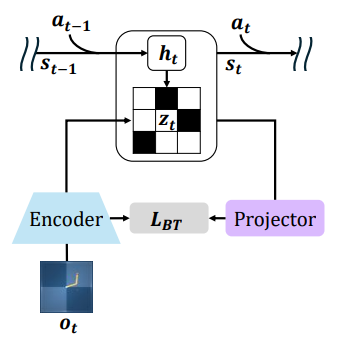
\includegraphics[width=0.5\textwidth]{figures/r2dreamer_arch.png}
    \caption{Representation learning in R2-Dreamer (figure obtained from \cite{morihira2026r2dreamer}). Instead of a decoder, a Projector component is used to align the latent state \( s_t \) with the embedding of the observation \( o_t \) through a Barlow Twins-style objective.}
    \label{fig:r2dreamer_arch}
\end{figure}

\section{Experimental Setup}

Our experiments go along two different axes: first, we evaluate the performance of R2-Dreamer on environments that we have previously worked with (Hopper-v3) in order to compare it with our baseline, and extend to similar but more complex ones (Walker2d-v3). Second, we evaluate the performance of R2-Dreamer on the CarRacing-v3 environment, which is a visual, continuous control task that we have not previously worked with, and where we expect the benefits of the world model to be more pronounced.

In Table~\ref{tab:hyperparams}, we summarize the main hyperparameters used in our experiments, which are based on the original R2-Dreamer implementation and adapted to our computational resources:

\begin{table}[H]
    \centering
    \caption{Essential hyperparameters for R2-Dreamer across different environments}
    \label{tab:hyperparams}
    \begin{tabular}{lccc}
        \hline
        \textbf{Parámetro}          & \textbf{walker\_walk} & \textbf{hopper\_hop} & \textbf{car\_racing2} \\
        \hline
        \texttt{action\_repeat}     & 2                     & 2                    & 4                     \\
        \texttt{time\_limit}        & 1000                  & 1000                 & 10000                 \\
        \texttt{steps}              & 1010000               & 1010000              & inf                   \\
        \texttt{batch\_size}        & 32                    & 16                   & 32                    \\
        \texttt{batch\_length}      & 32                    & 64                   & 32                    \\
        \texttt{imag\_horizon}      & 8                     & 15                   & 8                     \\
        \texttt{env\_num}           & 4                     & 4                    & 4                     \\
        \texttt{eval\_episode\_num} & 10                    & 10                   & 10                    \\
        \hline
    \end{tabular}
\end{table}

Apart from these, we use the same \textbf{learning rate} ($4 \times 10^{-5}$), \textbf{gradient clip} (1000.0) and \textbf{policy entropy coefficient} ($3 \times 10^{-4}$) across all environments, as they are the default values in the original implementation and we did not find it necessary to tune them for our experiments. Let's briefly explain the reasoning behind some of these hyperparameters:
\begin{itemize}
    \item \texttt{action\_repeat}: This parameter controls how many times the same action is repeated in the environment before taking a new action. In visual environments like CarRacing, a higher action repeat can help to reduce the frequency of decision-making and allow the agent to focus on more meaningful state transitions, while in simpler environments like Hopper and Walker, a lower action repeat can help to capture finer-grained dynamics (thus the difference between 2 and 4).
    \item \texttt{time\_limit}: This parameter sets the maximum number of steps per episode. In CarRacing, we set a higher time limit to allow the agent to explore the environment more thoroughly and learn from longer trajectories, while in Hopper and Walker, a lower time limit is sufficient to capture the relevant dynamics of the task (since these dynamics are much simpler and can be learned in shorter episodes).
    \item \texttt{steps}: This parameter constrains the total number of training steps. In CarRacing, we set it to infinity to allow the agent to train until convergence, while in Hopper and Walker, we set it to a fixed number (1 million) to ensure that the training process is manageable and does not take too long (and also to allow for a fair comparison with our baselines, which were trained for a similar number of steps).
    \item \texttt{imag\_horizon}: This parameter tunes the length of the imagined trajectories used for policy optimization. Since Hopper is a simpler environment with more deterministic dynamics, we can afford to use longer imagined trajectories (15 steps) without suffering from compounding errors, while in Walker and CarRacing, which are more complex and have more stochastic dynamics, we use shorter imagined trajectories (8 steps) to mitigate the impact of model inaccuracies.
\end{itemize}

\section{Results}

\section{Discussion}

\section{Conclusion}

\bibliographystyle{unsrtnat}
\bibliography{references}

\end{document}
